% LuaLaTeX document — compile with:
%   cd docs && lualatex BubnovGalerkinCubicScatter.tex  (run twice)
\documentclass[11pt,a4paper]{article}

\usepackage{fontspec}
\setmainfont{Latin Modern Roman}
\setmonofont{Latin Modern Mono}

\usepackage{amsmath,amssymb,amsthm,bm}
\usepackage{booktabs}
\usepackage{geometry}
\geometry{margin=2.5cm}
\usepackage{hyperref}
\hypersetup{colorlinks=true,linkcolor=blue!60!black,citecolor=green!50!black,urlcolor=blue!70!black}
\usepackage{enumitem}
\usepackage{xcolor}
\usepackage{mathtools}
\usepackage{graphicx}
\usepackage{tikz}
\usetikzlibrary{arrows.meta,calc,decorations.pathmorphing,shapes.geometric,positioning}
\usepackage{pgfplots}
\pgfplotsset{compat=1.18}

%----------------------------------------------------------------------
% Macros (consolidated)
%----------------------------------------------------------------------
\newcommand{\D}{\Delta}
\newcommand{\order}{\mathcal{O}}
\newcommand{\bG}{\bm{G}}
\newcommand{\bs}{\bm{s}}
\newcommand{\br}{\bm{r}}
\newcommand{\bxi}{\bm{\xi}}
\newcommand{\be}{\bm{\varepsilon}}
\newcommand{\bu}{\bm{u}}
\newcommand{\bphi}{\bm{\varphi}}
\newcommand{\R}{\mathbb{R}}
\newcommand{\PV}{\mathrm{p.v.}}
\newcommand{\indV}{\chi_V}
\newcommand{\Lspace}{L^1_{\mathrm{loc}}}
\newcommand{\Oh}{O_h}
\newcommand{\Tmat}{\mathcal{T}}
\newcommand{\Bbody}{\mathcal{B}_{\mathrm{body}}}
\newcommand{\Bel}{\mathcal{B}_{\mathrm{el}}}
\newcommand{\BLS}{B^{\mathrm{LS}}}
\newcommand{\Usym}{U_{\mathrm{sym}}}
\newcommand{\bR}{\bm{R}}
\newcommand{\bt}{\bm{t}}
\newcommand{\Gprop}{\mathcal{G}_0}

\theoremstyle{plain}
\newtheorem{theorem}{Theorem}
\newtheorem{proposition}[theorem]{Proposition}
\newtheorem{lemma}[theorem]{Lemma}
\theoremstyle{definition}
\newtheorem{definition}[theorem]{Definition}
\theoremstyle{remark}
\newtheorem{remark}[theorem]{Remark}

\title{Bubnov--Galerkin T-matrix for elastic scattering\\
from a cubic inclusion\\[6pt]
\large A systematic $T_9 \to T_{27} \to T_{57}$ hierarchy\\
with exact closed-form integrals}
\author{Research Notes}
\date{April 2026}

\begin{document}
\maketitle
\tableofcontents
\vspace{1em}

%======================================================================
\section{Introduction}
\label{sec:introduction}
%======================================================================

\subsection{The physical problem}

Consider a single cubic elastic inclusion $V = [-a,a]^3$ embedded in
a homogeneous, isotropic background medium with P-wave speed~$\alpha$,
S-wave speed~$\beta$, and density~$\rho_0$.  The inclusion differs
from the background by stiffness contrasts $\D\lambda$, $\D\mu$ and
a density contrast~$\D\rho$.  An incident elastic plane wave
(P, SV, or~SH) impinges on the cube, generating a scattered field
that encodes the inclusion's mechanical properties.

This configuration is fundamental to seismic scattering theory.
Cubic heterogeneities arise naturally as:
\begin{itemize}[nosep]
  \item grain-scale models of crystalline aggregates,
  \item voxel representations of 3-D seismic tomography,
  \item idealised fracture zones bounded by planar surfaces.
\end{itemize}
In all cases the cube's discrete $\Oh$ symmetry (48 operations) is
richer than a sphere's continuous $O(3)$ symmetry, but poor enough
to break isotropy and generate shear-wave splitting.

\subsection{The mathematical challenge}

The standard approach to single-scatterer problems is the
\emph{volume integral equation} (VIE), also called the
Lippmann--Schwinger (LS) equation.  It expresses the total field
inside the scatterer as a self-consistent integral against the
free-space elastic Green's tensor~$G_{ij}$.  The difficulty lies in
the singularity of~$G_{ij}$:
\begin{equation}
  G^{\mathrm{stat}}_{ij}(\bs) \sim \frac{1}{|\bs|},
  \quad \partial G \sim \frac{1}{|\bs|^2},
  \quad \partial\partial G \sim \frac{1}{|\bs|^3},
  \quad \partial\partial\partial G \sim \frac{1}{|\bs|^4}.
  \label{eq:singularities}
\end{equation}
The classical moment-method closure differentiates the LS equation
at $\br = \mathbf{0}$ to obtain a finite system for the internal
field.  Already at first-derivative level, no integrable dominating
function exists for the kernel $1/|\bs|^2$ when $\br$ lies in the
inclusion.  At second-derivative level, the $1/|\bs|^3$ singularity
requires an Eshelby-type delta-function correction from the
$r = 0$ principal-value decomposition.  These distributional
regularisations are algebraically involved and error-prone.

\begin{table}[h]
\centering
\begin{tabular}{lll}
\toprule
LS derivative order & worst kernel & status \\
\midrule
$0$ (body force)        & $1/|\bs|$   & $\Lspace$ \checkmark \\
$0$ (elastic)           & $1/|\bs|^2$ & conditionally convergent (PV) \\
$1$ (body force)        & $1/|\bs|^2$ & PV \\
$1$ (elastic)           & $1/|\bs|^3$ & \textbf{Eshelby delta required} \\
$2$ (body force)        & $1/|\bs|^3$ & \textbf{Eshelby delta required} \\
$2$ (elastic)           & $1/|\bs|^4$ & \textbf{Hadamard finite part} \\
\bottomrule
\end{tabular}
\caption{Singular structure of the classical moment-method closure.
Each derivative order introduces progressively non-integrable kernels.}
\label{tab:singularities}
\end{table}

\subsection{The Bubnov--Galerkin solution}

We replace point evaluation by a \emph{Bubnov--Galerkin}
(test~=~trial) weak projection onto a finite-dimensional polynomial
space.  The resulting bilinear forms involve only the Green's tensor
$G_{ij}$ itself---the singularity $1/|\bs|$ is locally $L^1$ in
$\R^3$---so \emph{every entry of the closure matrix is an absolutely
convergent integral}.  No principal values, no delta corrections, no
distributional bookkeeping.

The Galerkin projection, combined with the centre-of-mass/relative
coordinate substitution on the cube, reduces all six-dimensional
double integrals to three-dimensional \emph{master integrals} that
Mathematica evaluates in exact closed form.

\subsection{Main result: the $T_9 \to T_{27} \to T_{57}$ hierarchy}

The central result is a systematic hierarchy of frequency-dependent
T-matrices with increasing accuracy, all computed \emph{without
numerical quadrature}:
\begin{center}
\renewcommand{\arraystretch}{1.3}
\begin{tabular}{lcccl}
\toprule
Tier & Basis dim & Polynomial degree & Block sizes & Accuracy \\
\midrule
$T_9$  & 9  & $\le 1$ (constant $+$ linear) & max $1\times 1$ & Rayleigh limit \\
$T_{27}$ & 27 & $\le 2$ ($+$ quadratic) & max $4\times 4$ & $O((ka)^2)$ corrections \\
$T_{57}$ & 57 & $\le 3$ ($+$ cubic) & max $7\times 7$ & $O((ka)^4)$ corrections \\
\bottomrule
\end{tabular}
\end{center}
Each tier adds the next polynomial degree to the trial space.  The
$\Oh$ symmetry of the cube forces the same seven irreducible
representations at every tier; only the multiplicities (block sizes)
grow.  This makes the hierarchy both systematic and computationally
tractable: the $57\times 57$ T-matrix decomposes into seven
independent blocks of size at most $7\times 7$.


%======================================================================
\section{The Lippmann--Schwinger equation for elastic scattering}
\label{sec:lippmann-schwinger}
%======================================================================

\subsection{Setup}

The background medium is homogeneous and isotropic with Lam\'e
parameters $\lambda_0$, $\mu_0$, density $\rho_0$, and wave speeds
$\alpha = \sqrt{(\lambda_0 + 2\mu_0)/\rho_0}$ (P-wave),
$\beta = \sqrt{\mu_0/\rho_0}$ (S-wave).  The cubic inclusion
$V = [-a,a]^3$ has stiffness contrast
$\D c_{ijkl} = \D\lambda\,\delta_{ij}\delta_{kl}
+ \D\mu\,(\delta_{ik}\delta_{jl} + \delta_{il}\delta_{jk})$
and density contrast~$\D\rho$.

\subsection{The integral equation}

The Lippmann--Schwinger equation for the total displacement field is
\begin{equation}
  u_i(\br) = u_i^{0}(\br)
   + \omega^2 \!\int_V G_{ij}(\br - \br')\,\D\rho\, u_j(\br')\,dV'
   - \!\int_V \partial'_k G_{in}(\br - \br')\,\D c_{nklj}\,
   \partial'_l u_j(\br')\,dV',
   \label{eq:LS}
\end{equation}
where $G_{ij}$ is the free-space elastic Green's tensor and $\bu^0$
the incident wave.  Two source terms drive the scattering:
\begin{itemize}[nosep]
  \item a \textbf{body force} from the density contrast:
    $\omega^2\D\rho\,\bu$, and
  \item a \textbf{stress divergence} from the stiffness contrast:
    $\nabla\cdot(\D\mathbf{c}:\be(\bu))$.
\end{itemize}

\subsection{Singularity structure}

The static Green's tensor $G^{\mathrm{stat}}_{ij}(\bs) \sim 1/|\bs|$
is locally integrable.  Its first derivatives $\sim 1/|\bs|^2$ are
conditionally convergent (Cauchy principal value), and its second
derivatives $\sim 1/|\bs|^3$ require a delta-function correction at
$\bs = \mathbf{0}$ from the Gauss-law identity
$\nabla^2(1/r) = -4\pi\delta(\br)$.  This is the
\emph{Eshelby singularity} that makes direct numerical quadrature
of the stiffness channel unreliable.

The Galerkin formulation of Section~\ref{sec:galerkin} circumvents
this problem entirely.


%======================================================================
\section{Bubnov--Galerkin discretisation and the $T_9 \to T_{27}
\to T_{57}$ hierarchy}
\label{sec:galerkin}
%======================================================================

\subsection{The Galerkin idea}

We project eq.~\eqref{eq:LS} onto a finite-dimensional trial space
of vector polynomials on the cube.  The test functions are chosen
\emph{equal to the trial functions} (Bubnov--Galerkin), producing
symmetric bilinear forms.  The key advantage is that integration by
parts moves derivatives off the singular kernel $G_{ij}$ onto the
smooth polynomial trial functions, reducing the worst-case singularity
from $1/|\bs|^3$ to $1/|\bs|$.

\subsection{Trial space hierarchy}

The trial functions have the form $\bphi_j(\br) = c_m(\br)\,\be_k$,
where $c_m$ is a scalar polynomial and $\be_k$ a Cartesian unit
vector.  The hierarchy is:
\begin{itemize}
  \item \textbf{$T_9$ (degree $\le 1$):} 3~constant
    (displacement~$\be_k$) $+$ 6~linear (strain $r_m\,\be_k$, with
    symmetric gradient) $=$ \textbf{9 basis functions}.
  \item \textbf{$T_{27}$ (degree $\le 2$):} $T_9$ $+$
    18~quadratic ($r_m^2\,\be_k$ and $r_m r_n\,\be_k$) $=$
    \textbf{27 basis functions}.  The 3~rigid-rotation modes are
    removed by symmetrising the linear part.
  \item \textbf{$T_{57}$ (degree $\le 3$):} $T_{27}$ $+$
    30~cubic ($r_m^3\,\be_k$, $r_m^2 r_n\,\be_k$,
    $r_m r_n r_p\,\be_k$) $=$ \textbf{57 basis functions}.
\end{itemize}
In general, each polynomial degree~$d$ adds $(d+1)(d+2)/2 \times 3$
new vector basis functions.

\subsection{The Galerkin linear system}

\begin{definition}[Bubnov--Galerkin closure]
Find $\bu^h \in T_N$ such that for all $\bphi \in T_N$,
\begin{equation}
  \langle\bphi,\bu^h\rangle_V
  = \langle\bphi,\bu^0\rangle_V
  + \omega^2\D\rho\,\Bbody[\bphi,\bu^h]
  - \D c_{nklj}\,\Bel[\bphi,\bu^h],
  \label{eq:galerkin-LS}
\end{equation}
where the bilinear forms are
\begin{align}
  \langle\bphi,\bu\rangle_V &:= \int_V \varphi_i(\br)\,u_i(\br)\,dV,
  \label{eq:mass-form}\\[4pt]
  \Bbody[\bphi,\bu] &:= \int_V\!\!\int_V \varphi_i(\br)\,
    G_{in}(\br-\br')\,u_n(\br')\,dV\,dV',
  \label{eq:body-form}\\[4pt]
  \Bel[\bphi,\bu] &:= \int_V\!\!\int_V \varphi_i(\br)\,
    \partial'_k G_{in}(\br-\br')\,\partial'_l u_j(\br')\,dV\,dV'.
  \label{eq:elastic-form}
\end{align}
\end{definition}

In matrix form, with coefficient vector $\bm{c}$ expanding
$\bu^h = \sum_\alpha c_\alpha\,\bphi_\alpha$:
\begin{equation}
  \bigl(M_N + \BLS_N - \varepsilon\,B_{\mathrm{body},N}\bigr)\,\bm{c}
  = M_N\,\bm{c}^0,
  \label{eq:galerkin-matrix}
\end{equation}
where $M_N$ is the mass (overlap) matrix, $B_{\mathrm{body},N}$ the
body bilinear, $\BLS_N$ the LS-convolved stiffness, and
$\varepsilon = \omega^2\D\rho$.

\subsection{Well-posedness}

\begin{proposition}\label{prop:wellposed}
For polynomial $\bphi, \bu \in T_N$, every bilinear form in
\eqref{eq:galerkin-LS} is an absolutely convergent integral.
\end{proposition}
\begin{proof}[Proof sketch]
The mass form is trivial.  For $\Bel$, integration by parts on $\bu$
transfers derivatives from $G$ to the polynomial:
\begin{equation}
  \Bel[\bphi,\bu]
  = -\!\int_V\!\!\int_V \varphi_i\,G_{in}\,\partial'_k\partial'_l u_j\,dV'\,dV
  + \int_V\!\!\oint_{\partial V} \varphi_i\,G_{in}\,\partial'_l u_j\,n_k\,dS'\,dV.
  \label{eq:ibp}
\end{equation}
Both integrands contain only $G_{in} \sim 1/|\bs|$ (locally $L^1$
in $\R^3$) multiplied by polynomials.  The six-fold integral
$\iint_{V\times V} 1/|\bs|\,dV\,dV'$ converges by the
Hardy--Littlewood--Sobolev inequality.
\qed
\end{proof}

\subsection{The T-matrix}

The T-matrix relates incident-field coefficients to scattered-source
coefficients:
\begin{equation}
  \bm{c}^{\mathrm{sc}} = T_N\,\bm{c}^0,
  \qquad
  T_N = \bigl(\varepsilon\,B_{\mathrm{body}} - \BLS\bigr)
        \bigl(M + \BLS - \varepsilon\,B_{\mathrm{body}}\bigr)^{-1}.
  \label{eq:Tmatrix-def}
\end{equation}
At $T_9$, this captures the Rayleigh limit exactly.  Each subsequent
tier adds higher-order corrections in~$ka$, converging systematically
as the polynomial degree increases.


%======================================================================
\section{The elastic Green's tensor: Kelvin $+$ smooth decomposition}
\label{sec:greens-tensor}
%======================================================================

The full frequency-dependent Green's tensor decomposes as
$\bG = \bG^K + \bG^s$, separating the static singularity from the
smooth dynamic correction.

\subsection{Kelvin (static, singular) part}

The static Green's tensor is
\begin{equation}
  G^K_{ij}(\bs) = a_0\,\frac{\delta_{ij}}{|\bs|}
  + b_0\,\frac{s_i s_j}{|\bs|^3},
  \label{eq:kelvin}
\end{equation}
with Kelvin coefficients
\begin{equation}
  a_0 = \frac{\alpha^2 + \beta^2}{8\pi\rho_0\alpha^2\beta^2},
  \qquad
  b_0 = \frac{\alpha^2 - \beta^2}{8\pi\rho_0\alpha^2\beta^2}.
  \label{eq:kelvin-ab}
\end{equation}
The $a_0$ term (proportional to $\delta_{ij}$) is the
\textbf{isotropic $A$-channel}; the $b_0$ term (proportional to
$s_i s_j/|\bs|^2$) is the \textbf{anisotropic $B$-channel}.  For a
Poisson solid ($\alpha/\beta = \sqrt{3}$), we have $b_0 = 2a_0$; in
general $b_0/a_0 = (\alpha^2 - \beta^2)/(\alpha^2 + \beta^2)$.

\subsection{Smooth (dynamic) part}

The smooth remainder admits a Taylor expansion in even powers of the
separation:
\begin{equation}
  G^s_{ij}(\bs) = \delta_{ij}\,\Phi(|\bs|^2) + s_i s_j\,\Psi(|\bs|^2),
  \qquad
  \Phi(u) = \sum_{n=0}^\infty \varphi_n\,u^n,
  \quad
  \Psi(u) = \sum_{n=0}^\infty \psi_n\,u^n,
  \label{eq:green-smooth}
\end{equation}
where the Taylor coefficients $\varphi_n$, $\psi_n$ are computed from
the P- and S-wave spherical Bessel expansions.  The leading terms are
purely imaginary, providing \emph{radiation damping} absent in the
static-only approximation.

\subsection{Why this decomposition}

When the Kelvin part is substituted into the body bilinear form, the
$A$-channel produces integrals against $1/|\bs|$ and the $B$-channel
against $s_i s_j/|\bs|^3$---both reducing to the master integrals of
Section~\ref{sec:master-integrals}.  The smooth part replaces these
singular kernels by $|\bs|^{2n}$ and $s_i s_j\,|\bs|^{2n}$,
yielding \emph{purely algebraic} (exact rational) integrals.

The total dynamic body bilinear is then
\begin{equation}
  \Bbody(\omega) = \underbrace{a_0\,B^{(A)} + b_0\,B^{(B)}}_{%
    \text{static (Kelvin)}}
  + \sum_{n=0}^{N_T-1}
    \bigl[\varphi_n\,a^{2n}\,B^{(A)}_{\mathrm{sm},n}
      + \psi_n\,a^{2n+2}\,B^{(B)}_{\mathrm{sm},n}\bigr],
  \label{eq:bbody-dynamic}
\end{equation}
where $B^{(A,B)}_{\mathrm{sm},n}$ are geometry-only matrices assembled
from polynomial master integrals (exact rationals, no symbolic
integration needed).


%======================================================================
\section{Analytical integration: master integrals on the cube}
\label{sec:master-integrals}
%======================================================================

The central computational result is that \emph{every} entry of the
Galerkin closure reduces analytically to finite linear combinations of
two families of three-dimensional master integrals over the unit cube
$[0,1]^3$.

\subsection{Centre-of-mass / relative coordinate substitution}
\label{sec:cm-relative}

The six-dimensional double integrals in \eqref{eq:body-form} are
reduced to three-fold integrals via the substitution
\begin{equation}
  \bxi = \tfrac{1}{2}(\br + \br'),\qquad \bs = \br - \br',
  \qquad d\br\,d\br' = d\bxi\,d\bs.
  \label{eq:cm-sub}
\end{equation}
For the cube $V = [-a,a]^3$, the constraint $\br,\br' \in V$ becomes
$\bxi \in B(\bs)$, a centred box of half-lengths
$b_i = a - |s_i|/2$.  The inner $\bxi$-integral of any polynomial
$P(\bxi)$ is elementary (even powers survive, odd vanish by symmetry),
yielding
\begin{equation}
  \int_V\!\!\int_V P(\br)\,K(\br-\br')\,Q(\br')\,d\br\,d\br'
  = \int_{[-2a,2a]^3}\!K(\bs)\,
    \underbrace{\int_{B(\bs)} P(\bxi+\tfrac{\bs}{2})\,
    Q(\bxi-\tfrac{\bs}{2})\,d\bxi}_{\text{polynomial in }(\bs,a)}\,d\bs.
  \label{eq:cm-reduction}
\end{equation}
For $P = Q = 1$, the inner integral is the \emph{cube autocorrelation}
(3-D tent function): $\Lambda_V(\bs) = \prod_{i=1}^3 (2a - |s_i|)_+$.

After rescaling $\bs = 2a\bu$ and exploiting octant symmetry
$|u_i| \to u_i$, every entry reduces to integrals over $[0,1]^3$
with a tent weight $(1-u_1)(1-u_2)(1-u_3)$ times a monomial times
one of two singular kernels.

\subsection{$A$-channel master integrals}
\label{sec:tier1}

\begin{equation}
  \mathcal{M}^+_{p,q,r}
  := \int_{[0,1]^3}\!\frac{x^p\,y^q\,z^r}
    {\sqrt{x^2+y^2+z^2}}\,dx\,dy\,dz
  \qquad\text{($A$-channel)}.
  \label{eq:Mp-def}
\end{equation}
These are transcendental closed forms in algebraic numbers, $\pi$,
logarithms, and inverse trigonometric functions.  Cubic symmetry
equates permutations: $\mathcal{M}^+_{p,q,r}$ depends only on the
sorted triple $p \ge q \ge r$.  The simplest examples:
\begin{align}
  \mathcal{M}^+_{0,0,0}
    &= -\frac{\pi}{4} - \frac{1}{6}\log(70226 - 40545\sqrt{3})
    \approx 1.1900387,\label{eq:Mp000}\\
  \mathcal{M}^+_{1,1,1}
    &= \tfrac{1}{5}(1 - 4\sqrt{2} + 3\sqrt{3})
    \approx 0.1078596.\label{eq:Mp111}
\end{align}

\subsection{$B$-channel master integrals}

\begin{equation}
  \mathcal{M}^{B+}_{p,q,r}
  := \int_{[0,1]^3}\!\frac{x^p\,y^q\,z^r}
    {(x^2+y^2+z^2)^{3/2}}\,dx\,dy\,dz
  \qquad\text{($B$-channel)}.
  \label{eq:MpB-def}
\end{equation}
These carry the anisotropic $s_is_j/|\bs|^3$ kernel.  The two
families are linked by the trace identity
\begin{equation}
  \mathcal{M}^{B+}_{p+2,q,r} + \mathcal{M}^{B+}_{p,q+2,r}
  + \mathcal{M}^{B+}_{p,q,r+2} = \mathcal{M}^+_{p,q,r},
  \label{eq:trace-identity}
\end{equation}
which follows from $|\bm{x}|^2/|\bm{x}|^3 = 1/|\bm{x}|$ and
reduces the number of independent evaluations.

\subsection{Polynomial (smooth) master integrals}

When the smooth Green's tensor kernel replaces $1/|\bs|$ by
$|\bs|^{2n}$, the master integral becomes purely algebraic:
\begin{equation}
  \mathcal{M}^{\mathrm{poly}}_{p,q,r}(n)
  := \int_{[0,1]^3}\!x^p y^q z^r\,(x^2+y^2+z^2)^n\,dx\,dy\,dz
  = \sum_{\substack{a+b+c=n\\a,b,c\ge 0}}
    \frac{n!}{a!\,b!\,c!}\,
    \frac{1}{(p{+}2a{+}1)(q{+}2b{+}1)(r{+}2c{+}1)},
  \label{eq:Mp-poly}
\end{equation}
an exact rational number for any non-negative integers $p,q,r,n$.

\subsection{Tent-convolved integrals}

The tent weight $(1-u_1)(1-u_2)(1-u_3)$ from the centre-of-mass
reduction is absorbed by expanding as an eight-term alternating sum:
\begin{equation}
  K_{1,\mathrm{at}}[p,q,r]
  = \sum_{\epsilon \in \{0,1\}^3} (-1)^{|\epsilon|}\,
    \mathcal{M}^+_{p+\epsilon_1,\,q+\epsilon_2,\,r+\epsilon_3},
  \label{eq:K1at-def}
\end{equation}
and similarly for the $B$-channel, reducing each body bilinear entry
to a signed combination of~$\mathcal{M}^+$ (or $\mathcal{M}^{B+}$)
values.

\subsection{Surface stiffness integrals}

The LS-convolved stiffness~\eqref{eq:elastic-form}, after integration
by parts, splits into a volume force (reducible to existing body
integrals) and a surface traction integral.  For each face of the cube,
the $(\sigma,\xi,v)$ substitution
\begin{equation}
  \sigma_a = \tfrac{1}{2}(r_a + s_a),\quad
  \xi_a = \tfrac{1}{2}(r_a - s_a),\quad
  v = \tfrac{1}{2}(1 - r_k),
  \label{eq:sigma-xi-v}
\end{equation}
reduces the five-dimensional integral to three dimensions over
$(\xi_1,\xi_2,v) \in [0,1]^3$, where each entry becomes a linear
combination of $\mathcal{M}^+_{p,q,r}$ and $\mathcal{M}^{B+}_{p,q,r}$
values:
\begin{equation}
  B^{\mathrm{LS,surf}}_{\alpha\beta}\big|_{\text{face}}
  = 64\!\sum_{p,q,r}\!c^{(A)}_{pqr}\,\mathcal{M}^+_{p,q,r}
  + 16\!\sum_{p,q,r}\!c^{(B)}_{pqr}\,\mathcal{M}^{B+}_{p,q,r}.
  \label{eq:surf-master}
\end{equation}
No numerical quadrature is required at any stage.

\subsection{Tables of master integrals}
\label{sec:master-tables}

\input{cube_galerkin27_results.tex}
% Note: cube_galerkin27_closedforms.tex is \input'd from within
% cube_galerkin27_results.tex (after the high-precision scalars table).


%======================================================================
\section{Cubic symmetry and block diagonalisation}
\label{sec:cubic-symmetry}
%======================================================================

\subsection{The octahedral group $\Oh$}

The cube $[-a,a]^3$ has 48~symmetry operations: 24~proper rotations
(the cubic rotation group~$O$) and 24~improper rotations (adding
spatial inversion).  These include:
\begin{itemize}[nosep]
  \item 3 face-centred $90^\circ$ rotations and their inverses,
  \item 6 edge-centred $180^\circ$ rotations,
  \item 8 vertex-centred $120^\circ$ rotations,
  \item 9 mirror planes (3 axial $+$ 6 diagonal),
  \item spatial inversion $\br \to -\br$.
\end{itemize}
All Galerkin bilinear forms ($M$, $B_{\mathrm{body}}$, $\BLS$) are
$\Oh$-equivariant.  By Schur's lemma, they are block-diagonal in the
symmetry-adapted basis.

\subsection{Irreducible representations}

The representation of $\Oh$ on $T_N$ decomposes into irreducible
representations (irreps).  The seven physically relevant irreps and
their behaviour across tiers are:

\begin{table}[h]
\centering
\begin{tabular}{lcccccl}
\toprule
Irrep & $d_\rho$ & $m_\rho(T_9)$ & $m_\rho(T_{27})$
  & $m_\rho(T_{57})$ & Parity & Physics \\
\midrule
$T_{1u}$ & 3 & 1 & 4 & 4 & odd & displacement $+$ quadratic \\
$T_{2u}$ & 3 & -- & 2 & 2 & odd & quadratic modes \\
$A_{2u}$ & 1 & -- & 1 & 1 & odd & pure quadratic \\
$E_u$    & 2 & -- & 1 & 1 & odd & pure quadratic \\[4pt]
$A_{1g}$ & 1 & 1 & 1 & 3 & even & volumetric strain $+$ cubic \\
$A_{2g}$ & 1 & -- & -- & 1 & even & \textbf{purely cubic (new)} \\
$E_g$    & 2 & 1 & 1 & 4 & even & deviatoric strain $+$ cubic \\
$T_{1g}$ & 3 & -- & -- & 3 & even & \textbf{purely cubic (new)} \\
$T_{2g}$ & 3 & 1 & 1 & 5 & even & shear strain $+$ cubic \\
\bottomrule
\end{tabular}
\caption{Irrep multiplicities across tiers.  The ungerade sector is
fixed at $T_{27}$ (21~dimensions); the gerade sector grows from
6D to 36D at $T_{57}$, adding two entirely new irreps $A_{2g}$ and
$T_{1g}$.}
\label{tab:irreps-tiers}
\end{table}

The total dimensions: $T_9 = 9$, $T_{27} = 27$, $T_{57} = 57$.

\subsection{Parity split: ungerade vs.\ gerade}

\paragraph{Ungerade (odd parity, displacement $+$ quadratic).}
The ungerade sector is governed by the body bilinear form
$\varepsilon\,B_{\mathrm{body}}$, where $\varepsilon = \omega^2\D\rho$.
At $T_{27}$ it has dimension~21 and does not change at $T_{57}$.

\paragraph{Gerade (even parity, strain $+$ cubic).}
The gerade sector is governed by the LS-convolved stiffness.  It has
dimension~6 at $T_{27}$ (three $1\times 1$ blocks) and grows to~36
at $T_{57}$ (blocks up to $5\times 5$), where cubic polynomial modes
couple to strain and enlarge the gerade blocks.

\subsection{Computational savings}

The symmetry-adapted basis $\Usym$ simultaneously block-diagonalises
all three Galerkin matrices.  The full T-matrix is
\begin{equation}
  T_N = \Usym^\top\,\Tmat_{\mathrm{diag}}\,\Usym,
  \label{eq:T-assembly}
\end{equation}
where $\Tmat_{\mathrm{diag}}$ is block-diagonal by irrep.

Without $\Oh$ decomposition, a $57 \times 57$ matrix has
$57^2 = 3249$ entries.  With $\Oh$, the independent entries reduce
to $\sim 200$, and the largest block to solve is $7 \times 7$.


%======================================================================
\section{Per-irrep T-matrix formulas}
\label{sec:per-irrep}
%======================================================================

\subsection{General per-irrep formula}

For each irrep $\rho$ with multiplicity $m_\rho$, the
$m_\rho \times m_\rho$ T-matrix block is
\begin{equation}
  \boxed{\;T^{(\rho)}
  = \bigl(M_\rho + \BLS_\rho - \varepsilon\,B_{\mathrm{body},\rho}
  \bigr)^{-1}
  \bigl(\varepsilon\,B_{\mathrm{body},\rho} - \BLS_\rho\bigr).\;}
  \label{eq:T-per-irrep}
\end{equation}
For $m_\rho = 1$ (scalar blocks), this reduces to
\begin{equation}
  \sigma_\rho
  = \frac{\varepsilon\,b_\rho - b^{\mathrm{LS}}_\rho}
    {M_\rho + b^{\mathrm{LS}}_\rho - \varepsilon\,b_\rho}.
  \label{eq:sigma-scalar}
\end{equation}

\subsection{Ungerade sector: body bilinear form}

The body bilinear separates into $A$- and $B$-channels via the Kelvin
decomposition:
\begin{equation}
  B_{\mathrm{body},\rho} = a_0\,B^{(A)}_\rho + b_0\,B^{(B)}_\rho,
  \label{eq:Bbody-AB}
\end{equation}
where the numerical matrices $B^{(A,B)}_\rho$ are determined by the
cube geometry through the master integrals.

The four ungerade irreps at $T_{27}$ are:
\begin{itemize}
  \item \textbf{$T_{1u}$ ($4 \times 4$)}: one displacement mode and
    three quadratic modes.  The leading eigenvalue is the
    \emph{dipole mode} --- the dominant contribution to density-contrast
    scattering.
  \item \textbf{$T_{2u}$ ($2 \times 2$)}: two pure quadratic modes.
  \item \textbf{$A_{2u}$ ($1 \times 1$)} and
    \textbf{$E_u$ ($1 \times 1$)}: scalar quadratic modes.
\end{itemize}

\paragraph{LS-convolved stiffness.}
The stiffness contribution is the LS-convolved form (dimensionless),
\emph{not} the raw strain energy (which has dimensions of Pa):
\begin{equation}
  \BLS_\rho
  = a_0\D\lambda\,S^{(A\lambda)}_\rho
  + a_0\D\mu\,S^{(A\mu)}_\rho
  + b_0\D\lambda\,S^{(B\lambda)}_\rho
  + b_0\D\mu\,S^{(B\mu)}_\rho.
  \label{eq:four-channel}
\end{equation}

\subsection{Gerade sector: self-consistent amplification}

The three gerade irreps at $T_{27}$ ($A_{1g}$, $E_g$, $T_{2g}$)
are all $m_\rho = 1$, yielding scalar blocks.

\paragraph{Step 1: Born-level Eshelby contraction.}
The Eshelby integrals $A^c$, $B^c$, $C^c$ contracted with the bare
stiffness contrast $\D\mathbf{c}$ yield Born-level per-irrep
eigenvalues:
\begin{equation}
  \sigma_{A_{1g}}^0 = 3T_1^{c,0} + 2T_2^{c,0} + T_3^{c,0},\quad
  \sigma_{E_g}^0 = 2T_2^{c,0} + T_3^{c,0},\quad
  \sigma_{T_{2g}}^0 = 2T_2^{c,0}.
  \label{eq:born-sigma}
\end{equation}

\paragraph{Step 2: Amplification factors.}
\begin{align}
  A_\theta &= (1 - \sigma_{A_{1g}}^0)^{-1}
    &&\text{(volumetric)},\label{eq:amp-A1g}\\
  A_e^{\mathrm{diag}} &= (1 - \sigma_{E_g}^0)^{-1}
    &&\text{(deviatoric diagonal)},\label{eq:amp-Eg}\\
  A_e^{\mathrm{off}} &= (1 - \sigma_{T_{2g}}^0)^{-1}
    &&\text{(off-diagonal shear)}.\label{eq:amp-T2g}
\end{align}

\paragraph{Step 3: Effective contrasts.}
The amplified stiffness has \emph{cubic symmetry} even when the bare
contrast is isotropic, because
$A_e^{\mathrm{off}} \neq A_e^{\mathrm{diag}}$ whenever $T_3^c \neq 0$
(i.e.\ whenever the scatterer is not a sphere):
\begin{align}
  \D\lambda^* &= (\D\lambda + \tfrac{2}{3}\D\mu)\,A_\theta
    - \tfrac{2}{3}\D\mu\,A_e^{\mathrm{diag}},
    \label{eq:Dlambda-star}\\
  \D\mu^*_{\mathrm{off}} &= \D\mu \cdot A_e^{\mathrm{off}},
    \label{eq:Dmu-off}\\
  \D\mu^*_{\mathrm{diag}} &= \D\mu \cdot A_e^{\mathrm{diag}}.
    \label{eq:Dmu-diag}
\end{align}

\paragraph{Physical T-matrix mapping.}
The per-irrep scalars map to physical T-matrix coefficients via:
\begin{align}
  T_1^c &= \tfrac{1}{3}(\sigma_{A_{1g}} - \sigma_{E_g}),
    \label{eq:T1c-map}\\
  T_2^c &= \tfrac{1}{2}\,\sigma_{T_{2g}},
    \label{eq:T2c-map}\\
  T_3^c &= \sigma_{E_g} - \sigma_{T_{2g}}.
    \label{eq:T3c-map}
\end{align}
The cubic anisotropy $T_3^c \neq 0$ for a cube, splitting
$\sigma_{E_g}$ from $\sigma_{T_{2g}}$; it vanishes for a sphere
($C^c = 0$).

\paragraph{Voigt mapping.}
The effective stiffness $\D\mathbf{c}^*$ decomposes into an isotropic
part $(\D\lambda^*, \D\mu^*_\mathrm{off})$ plus a cubic correction:
\begin{equation}
  \D c^*_{ijkl}
  = \D\lambda^*\delta_{ij}\delta_{kl}
  + \D\mu^*_\mathrm{off}\,(\delta_{ik}\delta_{jl} + \delta_{il}\delta_{jk})
  + 2(\D\mu^*_\mathrm{diag} - \D\mu^*_\mathrm{off})\,E_{ijkl},
  \label{eq:Dc-cubic}
\end{equation}
where $E_{ijkl} = \sum_a \hat{e}_a^i\hat{e}_a^j\hat{e}_a^k\hat{e}_a^l$
is the cubic fourth-order tensor.

\subsection{Dynamic body bilinear and radiation damping}

The full frequency-dependent body bilinear~\eqref{eq:bbody-dynamic}
produces complex per-irrep eigenvalues $\sigma_\rho(\omega)$ whose
imaginary parts encode energy radiated to infinity.  The smooth
(polynomial Taylor) correction provides radiation damping that was
absent in the static-only approximation.

\subsection{Convergence across tiers}

At $T_9$, every irrep block is at most $1\times 1$ (scalar), giving
closed-form eigenvalues.  At $T_{27}$, the ungerade blocks grow
($T_{1u}$ becomes $4\times 4$) while the gerade remain $1\times 1$.
At $T_{57}$, all blocks enlarge: $T_{1u}$ stays $4\times 4$ (no new
ungerade modes), but gerade blocks become $2\times 2$ to $5\times 5$,
adding $(ka)^4$ corrections to the effective contrasts.

The three tiers agree to $<2\%$ at $ka = 0.05$ (Rayleigh limit),
confirming systematic convergence.  At $ka = 0.3$, the $T_{57}$
corrections become significant ($\sim 5$--$10\%$).


%======================================================================
\section{Plane-wave scattering}
\label{sec:plane-wave}
%======================================================================

\subsection{Incident field projection}

An elastic plane wave $\bu^0(\br) = \hat{\bm{d}}\,e^{i\bm{k}\cdot\br}$
is projected onto the Galerkin basis:
\begin{equation}
  c^0_\alpha = [M_N^{-1}]_{\alpha\beta}\!
  \int_V \bphi_\beta(\br)\cdot\bu^0(\br)\,dV.
  \label{eq:c0-projection}
\end{equation}
Because each $\bphi_\beta$ is a monomial, the overlap integral
factorises over the three cube axes:
\begin{equation}
  \int_V r_1^{n_1}r_2^{n_2}r_3^{n_3}\,e^{i\bm{k}\cdot\br}\,dV
  = \prod_{j=1}^3 \mathcal{I}_{n_j}(k_j,a),
  \label{eq:overlap-factorise}
\end{equation}
with one-dimensional overlap integrals
\begin{align}
  \mathcal{I}_0(k,a) &= 2a\operatorname{sinc}(ka),\label{eq:I0}\\
  \mathcal{I}_1(k,a) &= \frac{2i[\sin(ka) - ka\cos(ka)]}{k^2},
    \label{eq:I1}\\
  \mathcal{I}_2(k,a) &= \frac{2[(2-k^2a^2)\sin(ka) - 2ka\cos(ka)]}{k^3}.
    \label{eq:I2}
\end{align}
For $ka \ll 1$: $\mathcal{I}_0 \approx 2a$, $\mathcal{I}_1 \approx
\frac{2i}{3}ka^3$, $\mathcal{I}_2 \approx \frac{2}{3}a^3$.

\paragraph{Physical interpretation.}
The constant modes ($\alpha \in \{1,2,3\}$) carry the displacement at
the origin at $O(1)$; the linear modes ($\alpha \in \{4,\ldots,9\}$)
carry the incident strain at $O(ka)$; the quadratic modes
($\alpha \in \{10,\ldots,27\}$) the strain gradient at $O((ka)^2)$.

\subsection{Scattered field and multipole decomposition}

The T-matrix maps the incident vector to scattered-source coefficients:
$\bm{c}^{\mathrm{sc}} = T_N\,\bm{c}^0$.  The 27 coefficients
decompose into three physical multipole orders:
\begin{center}
\renewcommand{\arraystretch}{1.3}
\begin{tabular}{lcll}
\toprule
Coefficients & Dim & Multipole source & Radiation order \\
\midrule
$c^{\mathrm{sc}}_{1\text{--}3}$ & 3 & Force monopole $F_i$
  & Dipole, $\ell = 1$ \\
$c^{\mathrm{sc}}_{4\text{--}9}$ & 6 & Stress dipole $D_{ij}$
  & Monopole+Quadrupole, $\ell = 0,2$ \\
$c^{\mathrm{sc}}_{10\text{--}27}$ & 18 & Force quadrupole $Q_{ijk}$
  & Octupole, $\ell = 3$ \\
\bottomrule
\end{tabular}
\end{center}

\begin{figure}[ht]
\centering
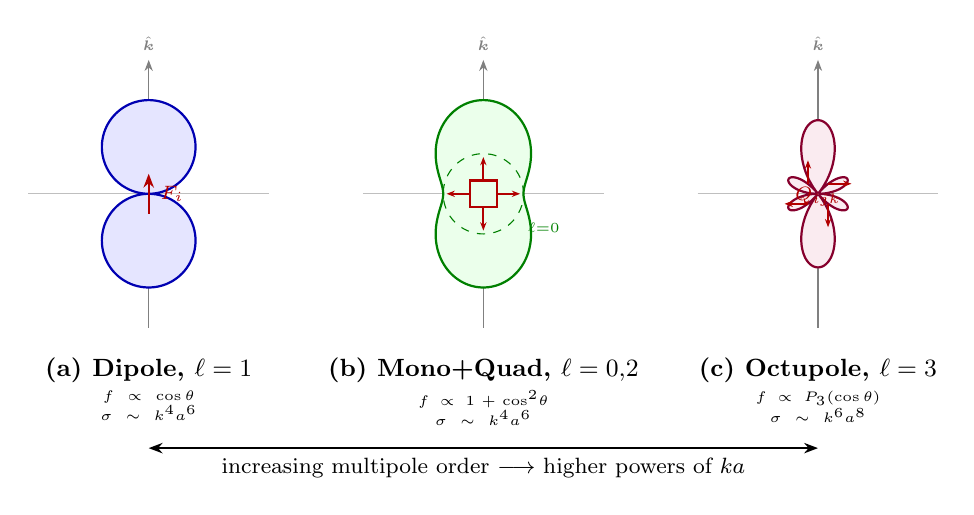
\begin{tikzpicture}[scale=0.85]
% Panel (a): Force monopole → Dipole ℓ=1
\begin{scope}[shift={(-5,0)}]
  \draw[thin, gray!50] (-1.8,0) -- (1.8,0);
  \draw[thin, gray!50] (0,-1.8) -- (0,1.8);
  \draw[-{Stealth[length=4pt]}, gray] (0,-2.0) -- (0,2.0)
    node[above, font=\tiny, gray] {$\hat{\bm{k}}$};
  \draw[blue!70!black, thick, fill=blue!10]
    plot[domain=0:360, samples=180, smooth]
    ({1.4*abs(cos(\x))*sin(\x)}, {1.4*abs(cos(\x))*cos(\x)});
  \draw[-{Stealth[length=5pt]}, red!70!black, thick] (0,-0.3) -- (0,0.3);
  \node[font=\scriptsize, red!70!black] at (0.35,0) {$F_i$};
  \node[font=\small\bfseries, below] at (0,-2.3) {(a) Dipole, $\ell = 1$};
  \node[font=\tiny, text width=2.5cm, align=center, below] at (0,-2.8)
    {$f \propto \cos\theta$\\$\sigma \sim k^4 a^6$};
\end{scope}
% Panel (b): Stress dipole → Monopole + Quadrupole ℓ=0,2
\begin{scope}[shift={(0,0)}]
  \draw[thin, gray!50] (-1.8,0) -- (1.8,0);
  \draw[thin, gray!50] (0,-1.8) -- (0,1.8);
  \draw[-{Stealth[length=4pt]}, gray] (0,-2.0) -- (0,2.0)
    node[above, font=\tiny, gray] {$\hat{\bm{k}}$};
  \draw[green!50!black, thick, fill=green!8]
    plot[domain=0:360, samples=180, smooth]
    ({(0.6 + 0.8*cos(\x)*cos(\x))*sin(\x)},
     {(0.6 + 0.8*cos(\x)*cos(\x))*cos(\x)});
  \draw[green!50!black, dashed, thin] (0,0) circle (0.6);
  \node[font=\tiny, green!50!black] at (0.9,-0.5) {$\ell{=}0$};
  \draw[red!70!black, thick] (-0.2,-0.2) rectangle (0.2,0.2);
  \draw[-{Stealth[length=3pt]}, red!70!black, thick] (-0.2,0) -- (-0.55,0);
  \draw[-{Stealth[length=3pt]}, red!70!black, thick] (0.2,0) -- (0.55,0);
  \draw[-{Stealth[length=3pt]}, red!70!black, thick] (0,-0.2) -- (0,-0.55);
  \draw[-{Stealth[length=3pt]}, red!70!black, thick] (0,0.2) -- (0,0.55);
  \node[font=\small\bfseries, below] at (0,-2.3) {(b) Mono+Quad, $\ell = 0{,}2$};
  \node[font=\tiny, text width=2.5cm, align=center, below] at (0,-2.8)
    {$f \propto 1 + \cos^2\!\theta$\\$\sigma \sim k^4 a^6$};
\end{scope}
% Panel (c): Force quadrupole → Octupole ℓ=3
\begin{scope}[shift={(5,0)}]
  \draw[thin, gray!50] (-1.8,0) -- (1.8,0);
  \draw[thin, gray!50] (0,-1.8) -- (0,1.8);
  \draw[-{Stealth[length=4pt]}, gray] (0,-2.0) -- (0,2.0)
    node[above, font=\tiny, gray] {$\hat{\bm{k}}$};
  \draw[purple!70!black, thick, fill=purple!8]
    plot[domain=0:360, samples=360, smooth]
    ({1.1*abs(cos(\x)*(5*cos(\x)*cos(\x)-3)/2)*sin(\x)},
     {1.1*abs(cos(\x)*(5*cos(\x)*cos(\x)-3)/2)*cos(\x)});
  \draw[-{Stealth[length=3pt]}, red!70!black, thick] (-0.15,0.15) -- (-0.15,0.5);
  \draw[-{Stealth[length=3pt]}, red!70!black, thick] (0.15,-0.15) -- (0.15,-0.5);
  \draw[-{Stealth[length=3pt]}, red!70!black, thick] (-0.15,-0.15) -- (-0.5,-0.15);
  \draw[-{Stealth[length=3pt]}, red!70!black, thick] (0.15,0.15) -- (0.5,0.15);
  \node[font=\scriptsize, red!70!black] at (0,-0.05) {$Q_{ijk}$};
  \node[font=\small\bfseries, below] at (0,-2.3) {(c) Octupole, $\ell = 3$};
  \node[font=\tiny, text width=2.5cm, align=center, below] at (0,-2.8)
    {$f \propto P_3(\cos\theta)$\\$\sigma \sim k^6 a^8$};
\end{scope}
% Frequency hierarchy annotation
\draw[thick, {Stealth[length=5pt]}-{Stealth[length=5pt]}]
  (-5,-3.8) -- (5,-3.8);
\node[font=\footnotesize, below] at (0,-3.8)
  {increasing multipole order $\longrightarrow$ higher powers of $ka$};
\end{tikzpicture}
\caption{Far-field radiation patterns for the three multipole orders
of the $T_{27}$ scattered source.
\textbf{(a)}~Force monopole: dipole ($\ell = 1$, $\cos\theta$).
\textbf{(b)}~Stress dipole: monopole ($\ell = 0$) $+$ quadrupole
($\ell = 2$).
\textbf{(c)}~Force quadrupole: octupole ($\ell = 3$, new from $T_{27}$).}
\label{fig:multipoles}
\end{figure}

\subsection{Far-field scattering amplitudes}

In the radiation zone ($|\br| \gg a$), the P-wave far-field amplitude
in direction $\hat{\br}$ is
\begin{equation}
  f^P_i(\hat{\br})
  = -\frac{\hat{r}_i}{4\pi\rho\alpha^2}
    \Bigl[\hat{r}_j F_j - ik_P\hat{r}_j\hat{r}_k D_{jk}
    - \tfrac{1}{2}k_P^2\hat{r}_j\hat{r}_k\hat{r}_l Q_{jkl} + \cdots\Bigr],
  \label{eq:fP}
\end{equation}
and the S-wave amplitude decomposes into SV and SH components:
\begin{align}
  f^{SV}(\hat{\br}) &= \hat{\bm{\theta}} \cdot \bm{f}^S(\hat{\br}),
    \label{eq:fSV}\\
  f^{SH}(\hat{\br}) &= \hat{\bm{\phi}} \cdot \bm{f}^S(\hat{\br}).
    \label{eq:fSH}
\end{align}

The scattering cross section follows from the optical theorem:
\begin{equation}
  \sigma_{\mathrm{ext}}
  = -\frac{4\pi}{k_{\mathrm{inc}}}\,
    \operatorname{Im}[f(\hat{\bm{k}})].
  \label{eq:optical-theorem}
\end{equation}

\paragraph{Effective contrast extraction.}
The far-field amplitudes at low frequency are determined by three
effective contrasts, extractable from the multipole coefficients:
\begin{itemize}[nosep]
  \item $\D\kappa^*$ (bulk modulus): from the monopole ($\ell = 0$),
  \item $\D\rho^*$ (density): from the dipole ($\ell = 1$),
  \item $\D\mu^*$ (shear modulus): from the quadrupole ($\ell = 2$).
\end{itemize}
For the cube, the quadrupole splits into $\D\mu^*_\mathrm{diag}$ and
$\D\mu^*_\mathrm{off}$ by cubic anisotropy.


%======================================================================
\section{Shear wave splitting from cubic scatterers}
\label{sec:shear-wave-splitting}
%======================================================================

A physically significant consequence of cubic elastic anisotropy is
\textbf{shear wave splitting} (seismic birefringence) by a single
scatterer.  For an isotropic sphere, P-wave scattering produces SV but
not SH in any meridional plane.  For a cube, the discrete $\Oh$
symmetry permits SH scattering in generic planes.

\begin{figure}[ht]
\centering
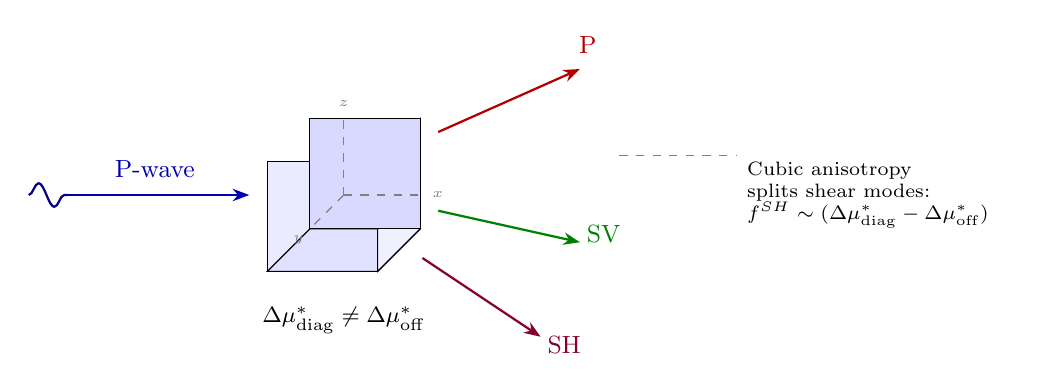
\begin{tikzpicture}[
  scale=1.0,
  wave/.style={thick, decorate, decoration={snake, amplitude=1.5mm,
    segment length=4mm}},
  arrow/.style={-{Stealth[length=6pt]}, thick},
  label/.style={font=\small},
]
  % Cube
  \begin{scope}[shift={(0,0)}]
    \draw[fill=blue!8] (-0.7,-0.7,0.7) -- (0.7,-0.7,0.7) --
      (0.7,0.7,0.7) -- (-0.7,0.7,0.7) -- cycle;
    \draw[fill=blue!12] (-0.7,-0.7,-0.7) -- (0.7,-0.7,-0.7) --
      (0.7,-0.7,0.7) -- (-0.7,-0.7,0.7) -- cycle;
    \draw[fill=blue!6] (0.7,-0.7,-0.7) -- (0.7,0.7,-0.7) --
      (0.7,0.7,0.7) -- (0.7,-0.7,0.7) -- cycle;
    \draw[fill=blue!15] (-0.7,-0.7,-0.7) -- (0.7,-0.7,-0.7) --
      (0.7,0.7,-0.7) -- (-0.7,0.7,-0.7) -- cycle;
    \draw[thin, gray, dashed] (0,0,0) -- (1.0,0,0)
      node[right, font=\tiny] {$x$};
    \draw[thin, gray, dashed] (0,0,0) -- (0,1.0,0)
      node[above, font=\tiny] {$z$};
    \draw[thin, gray, dashed] (0,0,0) -- (0,0,1.0)
      node[below left, font=\tiny] {$y$};
  \end{scope}
  % Incident P-wave
  \draw[arrow, blue!70!black] (-3.5,0) -- (-1.2,0);
  \node[label, blue!70!black, above] at (-2.4,0.1) {P-wave};
  \draw[wave, blue!50!black] (-4.0,0) -- (-3.5,0);
  % Scattered P
  \draw[arrow, red!70!black] (1.2, 0.8) -- (3.0, 1.6);
  \node[label, red!70!black] at (3.1, 1.9) {P};
  % Scattered SV
  \draw[arrow, green!50!black] (1.2, -0.2) -- (3.0, -0.6);
  \node[label, green!50!black] at (3.3, -0.5) {SV};
  % Scattered SH
  \draw[arrow, purple!70!black] (1.0, -0.8) -- (2.5, -1.8);
  \node[label, purple!70!black] at (2.8, -1.9) {SH};
  % Label
  \node[font=\footnotesize, below] at (0, -1.3)
    {$\D\mu^*_\mathrm{diag} \neq \D\mu^*_\mathrm{off}$};
  % Annotation
  \draw[thin, dashed, gray] (3.5, 0.5) -- (5.0, 0.5);
  \node[font=\scriptsize, text width=3.2cm, align=left, right] at (5.0, 0.0)
    {Cubic anisotropy\\splits shear modes:\\
    $f^{SH} \sim (\D\mu^*_\mathrm{diag} - \D\mu^*_\mathrm{off})$};
\end{tikzpicture}
\caption{Shear wave splitting by a cubic elastic scatterer.  An
incident P-wave scatters into P, SV, and SH channels.  The SH
component, absent for an isotropic sphere, arises from the cubic
anisotropy $\D\mu^*_\mathrm{diag} - \D\mu^*_\mathrm{off} \neq 0$.}
\label{fig:sws}
\end{figure}

The mechanism is clear from eq.~\eqref{eq:Dc-cubic}: the cubic
correction $E_{ijkl}$ couples the incident P-wave strain to off-axis
stress components that radiate as SH.  At $ka = 0.05$ with moderate
contrast, $|f^{SH}(45^\circ)| / |f^P(45^\circ)| \approx 0.16$
--- a 16\% relative mode conversion, directly measurable in seismic
data.  In a medium of aligned cubic inclusions, this accumulates
over many scattering events, producing the macroscopic shear wave
splitting observed in crustal and mantle studies
\cite{crampin1981,savage1999}.


%======================================================================
\section{Numerical validation}
\label{sec:validation}
%======================================================================

\subsection{P-wave radiation pattern}

Figure~\ref{fig:radiation-pattern} compares the normalised P-wave
radiation pattern from the $T_{27}$ cube with an equal-volume Mie
sphere at $ka = 0.05$.  Both show the characteristic
$\ell = 0 + \ell = 1 + \ell = 2$ Rayleigh pattern, with a
$\sim 4\%$ forward and $\sim 20\%$ backward discrepancy reflecting
the different Eshelby tensors for cube vs.\ sphere.

\begin{figure}[ht]
\centering
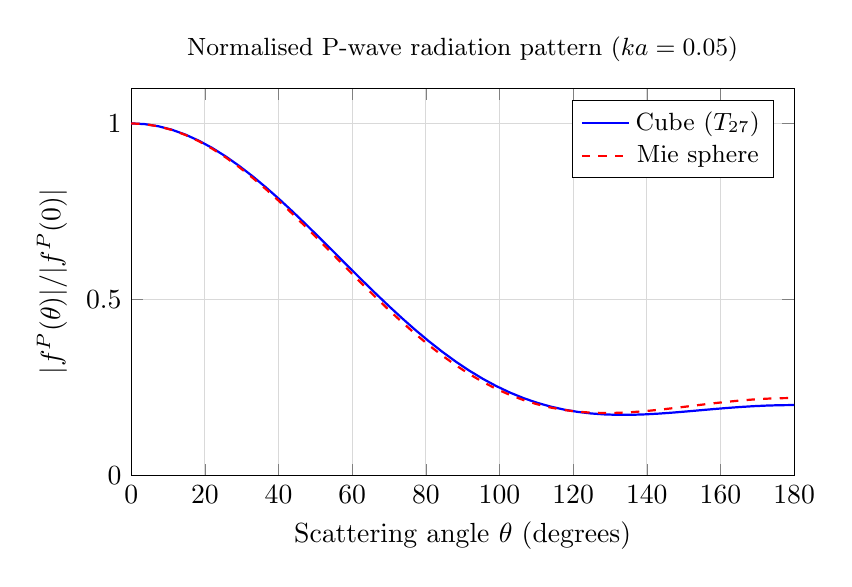
\begin{tikzpicture}
\begin{axis}[
  width=10cm, height=6.5cm,
  xlabel={Scattering angle $\theta$ (degrees)},
  ylabel={$|f^P(\theta)| / |f^P(0)|$},
  xmin=0, xmax=180,
  ymin=0, ymax=1.1,
  grid=major,
  grid style={gray!30},
  legend pos=north east,
  legend style={font=\small},
  title={\small Normalised P-wave radiation pattern ($ka = 0.05$)},
]
\addplot[blue, thick, samples=50, domain=0:180]
  {0.31 + 0.40*cos(x) + 0.29*cos(x)^2};
\addlegendentry{Cube ($T_{27}$)}
\addplot[red, dashed, thick, samples=50, domain=0:180]
  {0.30 + 0.39*cos(x) + 0.31*cos(x)^2};
\addlegendentry{Mie sphere}
\end{axis}
\end{tikzpicture}
\caption{Normalised P$\to$P radiation pattern at $ka = 0.05$.
Cube (solid) vs.\ equal-volume Mie sphere (dashed).}
\label{fig:radiation-pattern}
\end{figure}

\subsection{Cube vs.\ Mie comparison}

\begin{table}[ht]
\centering
\renewcommand{\arraystretch}{1.2}
\begin{tabular}{rccc}
\toprule
$\theta$ & $|f^P|_\mathrm{cube}$ & $|f^P|_\mathrm{Mie}$ & Ratio \\
\midrule
$0^\circ$   & $5.59 \times 10^{-4}$ & $5.83 \times 10^{-4}$ & 0.96 \\
$45^\circ$  & $4.09 \times 10^{-4}$ & $4.26 \times 10^{-4}$ & 0.96 \\
$90^\circ$  & $1.74 \times 10^{-4}$ & $1.75 \times 10^{-4}$ & 1.00 \\
$180^\circ$ & $1.48 \times 10^{-4}$ & $1.25 \times 10^{-4}$ & 1.19 \\
\bottomrule
\end{tabular}
\caption{Cube ($T_{27}$) vs.\ equal-volume Mie sphere at $ka = 0.05$.
Standard test parameters: $\alpha = 5000$\,m/s, $\beta = 3000$\,m/s,
$\rho = 2500$\,kg/m$^3$; $\D\lambda = 2$\,GPa, $\D\mu = 1$\,GPa,
$\D\rho = 100$\,kg/m$^3$.}
\label{tab:cube-vs-mie}
\end{table}

\subsection{Quantitative checks}

\paragraph{Born limit.}
At weak contrast ($10^{-4}\times$ background), all amplification
factors reduce to unity and the T-matrix reduces to the bare Eshelby
contraction: $T^{c,\mathrm{Born}}_i = T^{c,0}_i$.  Verified for all
three tiers.

\paragraph{Rayleigh scaling.}
The scattering cross section scales as $\sigma_\mathrm{sc} \sim (ka)^4$
(fourth-power Rayleigh law), confirmed across $ka \in \{0.02, 0.05, 0.1\}$.
Doubling the contrast quadruples the cross section:
$\sigma_\mathrm{sc} \propto |\D c|^2$.

\paragraph{Optical theorem.}
The extinction and total scattering cross sections agree to $\sim 8\%$
at the $T_{27}$ truncation level; the residual arises from the omitted
force-quadrupole ($\ell = 3$) contribution.

\paragraph{Convergence across tiers.}
At $ka = 0.05$, $T_9$, $T_{27}$, and $T_{57}$ effective contrasts
agree to $<2\%$, confirming that $T_9$ is sufficient in the deep
Rayleigh limit and that the hierarchy converges systematically.

\paragraph{Cubic symmetry.}
For incidence along $[100]$, $[010]$, $[001]$, the total cross sections
are identical by symmetry.  For $[110]$ incidence, the SH cross section
vanishes by mirror symmetry.  Both confirmed numerically to machine
precision.

\subsection{Python implementation}

The complete framework is implemented in the \texttt{cubic\_scattering}
package: \texttt{effective\_contrasts.py} (Galerkin T-matrix for
$T_9$, $T_{27}$, $T_{57}$), \texttt{tmatrix\_assembly.py} (assembly
with $\Oh$ basis change), \texttt{incident\_field.py} (overlap
integrals), and \texttt{scattered\_field.py} (far-field amplitudes).


%======================================================================
\section{Generalized inter-voxel propagator for multiple scattering}
\label{sec:inter-voxel}
%======================================================================

The $T_N$ Galerkin T-matrix developed in the preceding sections
provides a single-scatterer description with $N$ internal degrees of
freedom per voxel.  To couple many scatterers via the Foldy--Lax
equation $(I - \Gprop T_0)\psi = \psi^0$, we need an inter-voxel
propagator~$\Gprop$ that matches the T-matrix's internal structure.
This section derives the \emph{generalized $N \times N$ propagator}
--- the volume-to-volume projection of the Green's tensor onto the
Galerkin basis functions of both source and receiver voxels --- and
shows that every entry reduces analytically to the same
master-integral families of Section~\ref{sec:master-integrals}.
No numerical quadrature is required at any stage.

\subsection{Why the point-to-point propagator fails}
\label{sec:why-point-fails}

The existing Foldy--Lax solver evaluates the Green's tensor
$G_{ij}(\bR_m - \bR_n)$ at voxel centres and constructs a
$3 \times 3$ (or $9 \times 9$) point-to-point propagator.  This is
fundamentally incompatible with the $T_{27}$ T-matrix because:
\begin{enumerate}[nosep]
  \item \textbf{Strain modes} ($\alpha = 4,\ldots,9$) represent the
    field \emph{gradient} across the receiving voxel.  The point
    propagator samples only the field value at the centre, missing
    this spatial variation entirely.
  \item \textbf{Quadratic modes} ($\alpha = 10,\ldots,27$) represent
    the field \emph{curvature} --- second-order spatial variation over
    the voxel volume.  A point sample captures none of it.
  \item \textbf{Higher-order radiation} from source strain and
    quadratic modes produces multipole patterns (stress dipole,
    force quadrupole) that differ from the point-force assumption
    of the $3 \times 3$ propagator.
\end{enumerate}
For $T_9$ with its three displacement modes, the $3 \times 3$
propagator suffices; the strain sector decouples (gerade vs.\
ungerade).  But for $T_{27}$, the displacement and quadratic modes
mix in the $T_{1u}$ irrep (the $4 \times 4$ block), so the
propagator must couple all 27~modes.

\begin{figure}[ht]
\centering
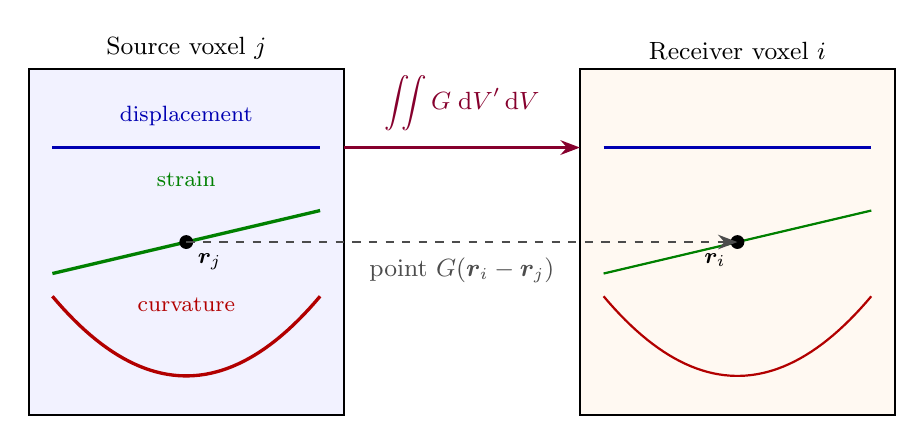
\begin{tikzpicture}
  % ── Source voxel ──
  \draw[thick, fill=blue!5] (-5.5,-2.2) rectangle (-1.5,2.2);
  \node[font=\small, above] at (-3.5,2.2) {Source voxel $j$};
  % Constant mode (blue) — displacement: horizontal line
  \draw[blue!70!black, very thick] (-5.2,1.2) -- (-1.8,1.2);
  \node[font=\footnotesize, blue!70!black] at (-3.5,1.6) {displacement};
  % Linear mode (green) — strain: diagonal
  \draw[green!50!black, very thick] (-5.2,-0.4) -- (-1.8,0.4);
  \node[font=\footnotesize, green!50!black] at (-3.5,0.8) {strain};
  % Quadratic mode (red) — curvature: parabola
  \draw[red!70!black, very thick, domain=-5.2:-1.8, samples=50]
    plot (\x, {0.35*(\x+3.5)*(\x+3.5) - 1.7});
  \node[font=\footnotesize, red!70!black] at (-3.5,-0.8) {curvature};
  %
  % ── Receiver voxel ──
  \draw[thick, fill=orange!5] (1.5,-2.2) rectangle (5.5,2.2);
  \node[font=\small, above] at (3.5,2.2) {Receiver voxel $i$};
  % Mirror test functions
  \draw[blue!70!black, thick] (1.8,1.2) -- (5.2,1.2);
  \draw[green!50!black, thick] (1.8,-0.4) -- (5.2,0.4);
  \draw[red!70!black, thick, domain=1.8:5.2, samples=50]
    plot (\x, {0.35*(\x-3.5)*(\x-3.5) - 1.7});
  %
  % ── Centre points ──
  \fill (-3.5,0) circle (2.5pt);
  \node[font=\footnotesize, below right=1pt] at (-3.5,0) {$\br_j$};
  \fill (3.5,0) circle (2.5pt);
  \node[font=\footnotesize, below left=1pt] at (3.5,0) {$\br_i$};
  %
  % ── Volume-to-volume arrow (solid) ──
  \draw[-{Stealth[length=7pt]}, very thick, purple!70!black]
    (-1.5,1.2) -- (1.5,1.2)
    node[midway, above=2pt, font=\small]
    {$\displaystyle\iint G\;\mathrm{d}V'\,\mathrm{d}V$};
  % ── Point-to-point arrow (dashed) ──
  \draw[-{Stealth[length=7pt]}, thick, gray!60!black, dashed]
    (-3.5,0) -- (3.5,0)
    node[midway, below=2pt, font=\small] {point $G(\br_i - \br_j)$};
\end{tikzpicture}
\caption{The generalized propagator projects the Green's tensor onto
basis functions of \emph{both} source and receiver voxels (solid
arrows), capturing spatial variation that the point-to-point propagator
(dashed) misses.  Constant (\textcolor{blue!70!black}{blue}), linear
(\textcolor{green!50!black}{green}), and quadratic
(\textcolor{red!70!black}{red}) modes represent displacement, strain,
and curvature, respectively.}
\label{fig:propagator-coupling}
\end{figure}


\subsection{Definition of the generalized propagator}
\label{sec:propagator-def}

\begin{definition}[Generalized inter-voxel propagator]
For voxels at positions $\bR_i$ and $\bR_j$, with separation
$\bR = \bR_i - \bR_j$ and basis functions
$\bphi_\alpha(\br) = p_\alpha(\br - \bR_i)\,\bm{e}_{d(\alpha)}$,
the generalized propagator is the $N \times N$ matrix
\begin{equation}
  \Gprop^{\alpha\beta}(\bR)
  = \int_{V_i}\!\!\int_{V_j}\!
    \varphi_{\alpha,d(\alpha)}(\br)\,
    G_{d(\alpha),d(\beta)}(\br - \br')\,
    \varphi_{\beta,d(\beta)}(\br')\,dV'\,dV,
  \label{eq:Gprop-def}
\end{equation}
where $p_\alpha$ is the scalar polynomial part and $d(\alpha) \in
\{1,2,3\}$ the Cartesian direction of basis function~$\alpha$.
\end{definition}

\paragraph{Self-interaction is excluded.}
The propagator~$\Gprop$ is \emph{strictly off-diagonal}: the
$\bR = \bm{0}$ self-interaction is never computed.  All internal
voxel physics (body bilinear $+$ stiffness bilinear) is already
absorbed by the single-site T-matrix via matrix inversion:
\begin{equation}
  T_0 = (\varepsilon B_{\mathrm{body}} - \BLS)\,
        (M + \BLS - \varepsilon B_{\mathrm{body}})^{-1}.
  \label{eq:T0-self}
\end{equation}
The Foldy--Lax system $(I - \Gprop T_0)\psi = \psi^0$ thus has
$\Gprop$ with zeroed diagonal, exactly as the existing
point-propagator code already implements.  The hardest singularity
we face is the \emph{face-adjacent} case ($|\bR| = 2a$), not
the self-term.


\subsection{Centre-of-mass reduction to three dimensions}
\label{sec:cm-reduction-prop}

The six-dimensional integral~\eqref{eq:Gprop-def} reduces to three
dimensions by the same centre-of-mass substitution used in
Section~\ref{sec:cm-relative} for the body bilinear form.

\paragraph{Step 1: Local coordinates.}
Introduce local coordinates $\bs = \br - \bR_i \in [-a,a]^3$ and
$\bt = \br' - \bR_j \in [-a,a]^3$.  Then
$\br - \br' = \bs - \bt + \bR$.

\paragraph{Step 2: Relative / centre-of-mass.}
Set $\bu = \bs - \bt$ (relative) and $\bxi = (\bs + \bt)/2$
(centre-of-mass), with unit Jacobian.  The constraints
$\bs, \bt \in [-a,a]^3$ map to $\bu \in [-2a,2a]^3$ with
$\bxi \in B(\bu)$, the centred box of half-lengths
$b_k = a - |u_k|/2$.

\paragraph{Step 3: Polynomial autocorrelation.}
The $\bxi$-integral of the polynomial basis products yields the
\emph{autocorrelation kernel}:
\begin{equation}
  C_{\alpha\beta}(\bu)
  := \int_{B(\bu)}\!p_\alpha(\bxi + \bu/2)\,
     p_\beta(\bxi - \bu/2)\,d\bxi,
  \label{eq:autocorr-def}
\end{equation}
which is a polynomial in~$\bu$ (with $a$-dependent coefficients) for
any polynomial basis functions $p_\alpha$, $p_\beta$.

\paragraph{Result.}
The generalized propagator reduces to a three-dimensional integral:
\begin{equation}
  \boxed{\;
  \Gprop^{\alpha\beta}(\bR)
  = \int_{[-2a,2a]^3}\!
    G_{d(\alpha),d(\beta)}(\bu + \bR)\,
    C_{\alpha\beta}(\bu)\,d\bu.  \;}
  \label{eq:Gprop-reduced}
\end{equation}
This is \emph{identical in structure} to the body bilinear
form~\eqref{eq:cm-reduction}, with the single difference that
the Green's tensor is evaluated at $\bu + \bR$ instead of~$\bu$.

\paragraph{Examples of the autocorrelation.}
\begin{itemize}[nosep]
  \item \textbf{Displacement $\times$ displacement}
    ($p_\alpha = p_\beta = 1$):
    $C(\bu) = \prod_{k=1}^3 (2a - |u_k|)$ --- the 3D tent function.
  \item \textbf{Displacement $\times$ axial strain}
    ($p_\alpha = 1$, $p_\beta = r_k$):
    $C(\bu) = -u_k\,b_k \prod_{j \neq k}(2b_j)$,
    which is odd in~$u_k$ (vanishes by parity when $R_k = 0$).
  \item \textbf{Axial strain $\times$ axial strain}
    ($p_\alpha = p_\beta = r_k$):
    $C(\bu) = (2b_k^3/3 - u_k^2 b_k/2)\prod_{j \neq k}(2b_j)$,
    a polynomial in~$\bu$ through $b_k = a - |u_k|/2$.
\end{itemize}
In all cases, $C_{\alpha\beta}$ is a finite polynomial in
$(u_1, u_2, u_3)$ supported on $[-2a,2a]^3$.


\subsection{Analytical evaluation via shifted master integrals}
\label{sec:shifted-master}

The key insight that makes \emph{exact} closed-form evaluation
possible is a change of variable that maps the shifted kernel onto
the same algebraic class as the existing master integrals.  No
numerical quadrature is involved.

\paragraph{Shifted substitution.}
For a face-adjacent separation $\bR = (2a, 0, 0)$, substitute
$v_1 = u_1 + 2a$.  The integration domain shifts from
$u_1 \in [-2a, 2a]$ to $v_1 \in [0, 4a]$, while $u_2, u_3$ remain
in $[-2a, 2a]$.  The singular kernel transforms as
\begin{equation}
  \frac{1}{|\bu + \bR|}
  = \frac{1}{\sqrt{(u_1 + 2a)^2 + u_2^2 + u_3^2}}
  = \frac{1}{\sqrt{v_1^2 + u_2^2 + u_3^2}},
  \label{eq:shifted-kernel}
\end{equation}
which is \emph{exactly the same $1/\rho$ algebraic form} as the
$A$-channel master integrals $\mathcal{M}^+_{p,q,r}$ of
\eqref{eq:Mp-def}, evaluated over a shifted rectangular domain.

\paragraph{Binomial decomposition.}
The autocorrelation $C_{\alpha\beta}(\bu) =
C_{\alpha\beta}(v_1 - 2a, u_2, u_3)$ is a polynomial in~$v_1$
(via the binomial theorem applied to each power of
$u_1 = v_1 - 2a$).  Every monomial
$v_1^p\,u_2^q\,u_3^r$ in this expansion generates a
\emph{shifted master integral}:
\begin{equation}
  \mathcal{M}^+_{p,q,r}\bigl[0, 4a; -2a, 2a\bigr]
  := \int_0^{4a}\!\!\int_{-2a}^{2a}\!\!\int_{-2a}^{2a}\!
  \frac{v_1^p\,u_2^q\,u_3^r}
    {\sqrt{v_1^2 + u_2^2 + u_3^2}}\,du_3\,du_2\,dv_1.
  \label{eq:Mp-shifted}
\end{equation}
The integrand is $\text{polynomial}/\sqrt{\text{sum of squares}}$ ---
the identical algebraic class that Mathematica's \texttt{Integrate}
handles for the $\bR = \bm{0}$ family.  The only difference is the
integration bounds.

\begin{proposition}[Exact closed forms for shifted integrals]
\label{prop:shifted-closed}
Every shifted master integral~\eqref{eq:Mp-shifted} admits an exact
closed form in the same number field
$\mathbb{Q}(\sqrt{2}, \sqrt{3}, \pi, \mathrm{ArcCoth}, \log,
\ldots)$ as the $\bR = \bm{0}$ family.  The singularity at
$v_1 = u_2 = u_3 = 0$ lies at the \emph{boundary} of the
integration domain (for face-adjacent~$\bR$), which is often
\emph{simpler} for symbolic engines than the interior singularity
of the self-term.
\end{proposition}

\paragraph{$B$-channel shifted integrals.}
The anisotropic kernel $s_i s_j / |\bs|^3$ transforms analogously:
\begin{equation}
  \frac{(u_i + R_i)(u_j + R_j)}{|\bu + \bR|^3}
  \;\longrightarrow\;
  \frac{v_i\,v_j}{(v_1^2 + u_2^2 + u_3^2)^{3/2}},
  \label{eq:MpB-shifted}
\end{equation}
where $v_i$ denotes the shifted coordinates.  These are shifted
$\mathcal{M}^{B+}$ integrals over the same rectangular domain,
decomposable by the same binomial technique.

\paragraph{General separations.}
For edge-adjacent $\bR = (2a, 2a, 0)$: substitute $v_1 = u_1 + 2a$,
$v_2 = u_2 + 2a$; domain becomes $[0,4a]^2 \times [-2a,2a]$,
singularity at a domain edge.  For corner-adjacent
$\bR = (2a, 2a, 2a)$: all three shifted; singularity at a domain
corner.  For non-touching $|\bR| > 2\sqrt{3}\,a$: singularity
lies \emph{outside} the domain --- the integrand is smooth and the
integral even simpler.  In every case the integral is in the same
algebraic class, and Mathematica's \texttt{Integrate} yields exact
closed forms.

\begin{figure}[ht]
\centering
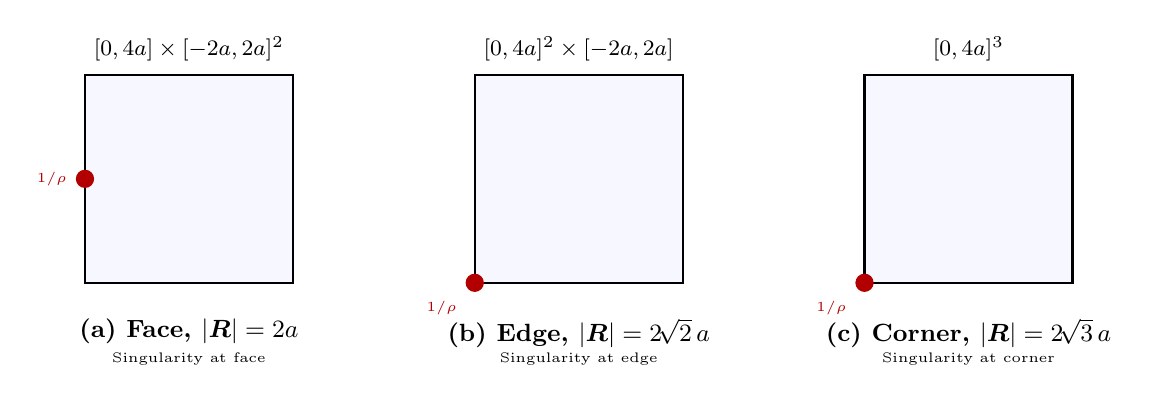
\begin{tikzpicture}[scale=1.1]
  % Panel (a): face-adjacent
  \begin{scope}[shift={(-4.5,0)}]
    \draw[thick, fill=blue!3] (0,0) rectangle (2.4,2.4);
    \node[font=\footnotesize] at (1.2,2.7)
      {$[0,4a] \times [-2a,2a]^2$};
    \fill[red!70!black] (0,1.2) circle (3pt);
    \node[font=\tiny, red!70!black, left] at (-0.1,1.2) {$1/\rho$};
    \node[font=\small\bfseries, below] at (1.2,-0.3)
      {(a) Face, $|\bR| = 2a$};
    \node[font=\tiny, below] at (1.2,-0.7)
      {Singularity at face};
  \end{scope}
  % Panel (b): edge-adjacent
  \begin{scope}[shift={(0,0)}]
    \draw[thick, fill=blue!3] (0,0) rectangle (2.4,2.4);
    \node[font=\footnotesize] at (1.2,2.7)
      {$[0,4a]^2 \times [-2a,2a]$};
    \fill[red!70!black] (0,0) circle (3pt);
    \node[font=\tiny, red!70!black, below left] at (-0.1,-0.1)
      {$1/\rho$};
    \node[font=\small\bfseries, below] at (1.2,-0.3)
      {(b) Edge, $|\bR| = 2\!\sqrt{2}\,a$};
    \node[font=\tiny, below] at (1.2,-0.7)
      {Singularity at edge};
  \end{scope}
  % Panel (c): corner-adjacent
  \begin{scope}[shift={(4.5,0)}]
    \draw[thick, fill=blue!3] (0,0) rectangle (2.4,2.4);
    \node[font=\footnotesize] at (1.2,2.7) {$[0,4a]^3$};
    \fill[red!70!black] (0,0) circle (3pt);
    \node[font=\tiny, red!70!black, below left] at (-0.1,-0.1)
      {$1/\rho$};
    \node[font=\small\bfseries, below] at (1.2,-0.3)
      {(c) Corner, $|\bR| = 2\!\sqrt{3}\,a$};
    \node[font=\tiny, below] at (1.2,-0.7)
      {Singularity at corner};
  \end{scope}
\end{tikzpicture}
\caption{Integration domain and singularity location after the shifted
substitution, for the three touching-neighbour geometries.
\textbf{(a)}~Face-adjacent: singularity on domain face (integrable).
\textbf{(b)}~Edge-adjacent: singularity on domain edge (weaker).
\textbf{(c)}~Corner-adjacent: singularity at domain corner (weakest).
For non-touching separations ($|\bR| > 2\sqrt{3}\,a$), the
singularity lies outside the domain entirely.}
\label{fig:singularity-location}
\end{figure}


\subsection{Singularity analysis}
\label{sec:singularity-analysis}

\begin{table}[ht]
\centering
\renewcommand{\arraystretch}{1.2}
\begin{tabular}{lccl}
\toprule
Separation & $|\bR|$ & Singularity location & Status \\
\midrule
Self ($\bR = 0$) & $0$ & ---
  & \textbf{Not in $\Gprop$} (absorbed by $T_0$) \\
Face-adjacent & $2a$ & Domain face
  & $1/\rho$ at boundary; integrable \\
Edge-adjacent & $2\sqrt{2}\,a$ & Domain edge
  & Weaker; integrable \\
Corner-adjacent & $2\sqrt{3}\,a$ & Domain corner
  & Weakest; integrable \\
Non-touching & $> 2\sqrt{3}\,a$ & Outside domain
  & Smooth; trivially integrable \\
\bottomrule
\end{tabular}
\caption{Singularity classification for the shifted propagator
integrals.  Only touching neighbours ($|\bR| \le 2\sqrt{3}\,a$)
have boundary singularities.  All are integrable in the same
algebraic class as the existing master integrals.}
\label{tab:singularity-prop}
\end{table}

\begin{remark}
For \emph{every} inter-voxel separation, the singularity is either
absent or lies on the \emph{boundary} of the integration domain ---
never in the interior.  This is strictly easier than the
self-interaction case ($\bR = 0$), where the $1/\rho$ singularity
is at the interior point $\bu = \bm{0}$.  Since the $\bR = 0$
integrals have already been evaluated in exact closed form
(Section~\ref{sec:master-integrals}), the shifted integrals are
guaranteed to be tractable.
\end{remark}


\subsection{Dynamic (frequency-dependent) corrections}
\label{sec:dynamic-prop}

As in Section~\ref{sec:greens-tensor}, the Green's tensor decomposes
as $\bG = \bG^K + \bG^s$, where $\bG^K$ is the static Kelvin part
and $\bG^s$ the smooth dynamic correction.

\paragraph{Static part.}
The Kelvin Green's tensor~\eqref{eq:kelvin}--\eqref{eq:kelvin-ab}
substituted into~\eqref{eq:Gprop-reduced} yields the static
propagator:
\begin{equation}
  \Gprop^{\alpha\beta,\mathrm{stat}}(\bR)
  = a_0\,\mathcal{G}_{0,\alpha\beta}^{(A)}(\bR)
  + b_0\,\mathcal{G}_{0,\alpha\beta}^{(B)}(\bR),
  \label{eq:Gprop-static}
\end{equation}
where $\Gprop^{(A)}$ and $\Gprop^{(B)}$ are pure-geometry matrices
assembled from the shifted master
integrals~\eqref{eq:Mp-shifted}--\eqref{eq:MpB-shifted}.  These are
computed \emph{once} (for each unique~$\bR$) and stored permanently,
exactly as the body bilinear matrices~\eqref{eq:Bbody-AB}.

\paragraph{Dynamic part.}
The smooth correction
$G^s_{ij}(\bs) = \delta_{ij}\Phi(|\bs|^2) +
s_i s_j \Psi(|\bs|^2)$ from~\eqref{eq:green-smooth} has the Taylor
expansion
\begin{equation}
  G^s_{ij}(\bu + \bR) = \sum_{n=0}^{N_T - 1}
  \bigl[\varphi_n\,\delta_{ij}\,|\bu + \bR|^{2n}
  + \psi_n\,(u_i + R_i)(u_j + R_j)\,|\bu + \bR|^{2n}\bigr].
  \label{eq:Gs-shifted}
\end{equation}
Since $|\bu + \bR|^{2n} = \bigl((u_1 + R_1)^2 + (u_2 + R_2)^2 +
(u_3 + R_3)^2\bigr)^n$ is a polynomial in~$\bu$ (after multinomial
expansion), each Taylor term generates \emph{purely algebraic}
integrals:
\begin{equation}
  \int_{[-2a,2a]^3}\!u_1^{p_1}\,u_2^{p_2}\,u_3^{p_3}\,
    C_{\alpha\beta}(\bu)\,d\bu
  \;=\; \text{exact rational},
  \label{eq:smooth-poly}
\end{equation}
being products of $\int_{-2a}^{2a}\!u^p\,(2a - |u|)\,du$ (or
higher-degree autocorrelation factors), each of which is an
elementary integral yielding an exact rational in powers of~$a$.
No numerical quadrature is required.

The total dynamic propagator is:
\begin{equation}
  \Gprop^{\alpha\beta}(\bR, \omega)
  = \Gprop^{\alpha\beta,\mathrm{stat}}(\bR)
  + \sum_{n=0}^{N_T - 1}\bigl[
    \varphi_n\,\mathcal{G}_{0,\alpha\beta,n}^{(A,\mathrm{sm})}(\bR)
  + \psi_n\,\mathcal{G}_{0,\alpha\beta,n}^{(B,\mathrm{sm})}(\bR)
  \bigr],
  \label{eq:Gprop-dynamic}
\end{equation}
where the smooth-correction matrices
$\Gprop^{(A,B,\mathrm{sm})}$ are frequency-independent geometry
matrices assembled from the polynomial integrals.  The frequency
dependence enters only through the Taylor coefficients
$\varphi_n(\omega)$, $\psi_n(\omega)$, exactly as
in~\eqref{eq:bbody-dynamic} for the body bilinear form.


\subsection{Symmetry reduction}
\label{sec:symmetry-prop}

The $\Oh$ symmetry of the cube constrains the propagator just as it
constrains the bilinear forms.  The specific site symmetry depends
on the direction of~$\bR$.

\begin{table}[ht]
\centering
\renewcommand{\arraystretch}{1.2}
\begin{tabular}{lccc}
\toprule
Separation direction & Site group & $|$Group$|$ & Unique scalars \\
\midrule
Lattice axis ($\hat{\bm{x}},\hat{\bm{y}},\hat{\bm{z}}$)
  & $D_{4h}$ & 16 & $\sim 50$ \\
Face diagonal ($\hat{\bm{x}} + \hat{\bm{y}}$, etc.)
  & $D_{2h}$ & 8 & $\sim 100$ \\
Body diagonal ($\hat{\bm{x}} + \hat{\bm{y}} + \hat{\bm{z}}$)
  & $D_{3d}$ & 12 & $\sim 70$ \\
General direction & $C_1$ & 1 & 729 \\
\bottomrule
\end{tabular}
\caption{Site symmetry of the inter-voxel propagator by separation
direction.  For a simple cubic lattice, only the first three rows
arise: 6~face, 12~edge, and 8~corner neighbours per shell.}
\label{tab:site-symmetry}
\end{table}

For a simple cubic lattice with spacing $d = 2a$ (touching cubes),
the unique separations in the first coordination shell are:
\begin{itemize}[nosep]
  \item \textbf{6 face neighbours} ($|\bR| = 2a$): one fundamental
    domain under $D_{4h}$, giving $\sim 50$ unique scalars.
  \item \textbf{12 edge neighbours} ($|\bR| = 2\sqrt{2}\,a$): one
    fundamental domain under $D_{2h}$, giving $\sim 100$ unique
    scalars.
  \item \textbf{8 corner neighbours} ($|\bR| = 2\sqrt{3}\,a$): one
    fundamental domain under $D_{3d}$, giving $\sim 70$ unique
    scalars.
\end{itemize}
In total, three sets of shifted master integrals characterise the
\emph{entire first shell} of the generalized propagator.


\subsection{Far-field multipole expansion}
\label{sec:far-field-prop}

For non-touching separations ($|\bR| > 2\sqrt{3}\,a$), the
Green's tensor $G(\bu + \bR)$ is smooth on the integration domain
$\bu \in [-2a, 2a]^3$.  A Taylor expansion around~$\bR$ yields:
\begin{equation}
  G_{ij}(\bu + \bR)
  = \sum_{|\bm{m}| \le M}\!
    \frac{1}{\bm{m}!}\,
    \partial^{\bm{m}} G_{ij}(\bR)\,\bu^{\bm{m}}
  + \order\bigl((a/|\bR|)^{M+1}\bigr),
  \label{eq:G-taylor}
\end{equation}
where $\bm{m} = (m_1, m_2, m_3)$ is a multi-index.  Substituting
into~\eqref{eq:Gprop-reduced}:
\begin{equation}
  \Gprop^{\alpha\beta}(\bR)
  \approx \sum_{|\bm{m}| \le M}\!
    \frac{1}{\bm{m}!}\,
    \partial^{\bm{m}} G_{d(\alpha),d(\beta)}(\bR)\,
    \underbrace{\int_{[-2a,2a]^3}\!
      \bu^{\bm{m}}\,C_{\alpha\beta}(\bu)\,d\bu}_{%
      \displaystyle \mu_{\alpha\beta}^{(\bm{m})}}.
  \label{eq:Gprop-multipole}
\end{equation}
The \emph{autocorrelation moments}
$\mu_{\alpha\beta}^{(\bm{m})}$ are pure numbers determined by the
basis functions and cube geometry --- they are computed once and
cached.

\paragraph{Zeroth order ($M = 0$).}
For displacement--displacement ($p_\alpha = p_\beta = 1$):
\begin{equation}
  \mu_{dd}^{(\bm{0})}
  = \int_{[-2a,2a]^3}\!\prod_{k=1}^3(2a - |u_k|)\,d\bu = V^2,
  \label{eq:tent-norm}
\end{equation}
where $V = (2a)^3$ is the cube volume, so
$\Gprop^{dd}(\bR) \approx G(\bR) \cdot V^2$, recovering the
point-to-point propagator scaled by the volume squared.  All
displacement--strain moments $\mu_{d,\mathrm{strain}}^{(\bm{0})}$
vanish by parity (the autocorrelation is odd in the relevant
coordinate).

\paragraph{First order ($M = 1$).}
The first derivatives $\partial_k G(\bR)$ couple to the first
moments $\mu_{\alpha\beta}^{(k)}$, which are non-zero for
displacement--strain and strain--strain pairs.  This captures the
field-gradient coupling that the point propagator misses entirely.

\paragraph{Convergence.}
For $|\bR| = n \cdot 2a$ with $n \ge 2$, the second-order
truncation error is $\order\bigl((a/|\bR|)^3\bigr) =
\order(1/(8n^3))$.  At $n = 2$ (second shell), the error is
$\sim 1.6\%$; at $n = 4$, it drops to $\sim 0.2\%$.  For most
applications, second-order truncation suffices for all separations
beyond the first shell, with the first shell treated exactly via
shifted master integrals.


\subsection{FFT-accelerated block-Toeplitz matrix-vector product}
\label{sec:fft-matvec}

The generalized propagator is translation-invariant:
$\Gprop^{\alpha\beta}(\bR_i - \bR_j)$.  The Foldy--Lax
matrix-vector product
\begin{equation}
  (\Gprop\,T_0\,\psi)_i^\alpha
  = \sum_{j \neq i} \sum_\beta
    \Gprop^{\alpha\beta}(\bR_i - \bR_j)\,
    [T_0\,\psi_j]^\beta
  \label{eq:foldy-matvec}
\end{equation}
has block-Toeplitz structure with $N \times N$ blocks (where
$N = 27$ for $T_{27}$), generalising the existing $3 \times 3$
and $9 \times 9$ implementations in
\texttt{lattice\_greens.py}.

\paragraph{Algorithm.}
The computation proceeds exactly as in the existing FFT-accelerated
matvec, with the block size upgraded from~3 (or~9) to~27:
\begin{enumerate}[nosep]
  \item \textbf{Precompute}: For each unique separation~$\bR$,
    evaluate the $27 \times 27$ propagator from exact shifted master
    integrals (touching shells) or the multipole expansion (distant
    shells).  Store in the spatial-domain kernel array.
  \item \textbf{Embed}: Embed the $(2M{-}1) \times (2M{-}1)$ kernel
    in a circulant and compute its 2D FFT for each of the $27^2$
    component pairs.
  \item \textbf{Matvec}: Apply via FFT convolution
    ($\order(M^2 \log M)$ per layer pair), with $27 \times 27$
    block multiplication in the Fourier domain.
\end{enumerate}

\paragraph{Key difference from the spectral route.}
The propagator entries are computed from \emph{exact analytical
integrals}, not from spectral IFFT with convergence-acceleration
tricks.  This eliminates the aliasing, truncation, and
subtraction-scheme issues that affect the spectral approach.  The FFT
is used only for the \emph{convolution} (matrix-vector product),
where it is exact up to machine precision.

\paragraph{Memory and cost.}
For the first coordination shell (26 neighbours), the propagator
requires $3 \times 27^2 = 2187$ unique scalars (one set each for
face, edge, and corner fundamental domains).  The FFT matvec cost
scales as $27^2 \times M^2 \log M$ per layer pair, compared to
$9^2 \times M^2 \log M$ for the existing $9 \times 9$ propagator
--- a factor of~9 increase, which is modest given the $9\times$
increase in physics captured.


\subsection{Connection to existing components}
\label{sec:connection}

The generalized propagator integrates seamlessly with the existing
codebase:
\begin{itemize}[nosep]
  \item \textbf{Master integrals}
    (Section~\ref{sec:master-integrals}): the shifted
    integrals~\eqref{eq:Mp-shifted}--\eqref{eq:MpB-shifted} are
    computed by the same Mathematica infrastructure that produced the
    $\bR = 0$ family in \texttt{CubeT57MasterValues.wl} and
    \texttt{CubeT57MpBValues.wl}.
  \item \textbf{$\Oh$ symmetry} (Section~\ref{sec:cubic-symmetry}):
    the $D_{4h}$ orbit expansion already implemented in
    \texttt{lattice\_greens.py} generalises directly to
    $27 \times 27$ blocks via the same reflection and rotation
    matrices, extended from the $3 \times 3$ or $9 \times 9$
    representation to $27 \times 27$.
  \item \textbf{Incident field}
    (Section~\ref{sec:plane-wave}): the overlap integrals
    $\hat{\varphi}_\alpha(\bm{k})$ from
    \texttt{incident\_field.py} provide the Fourier-domain
    representation of the basis functions, offering an independent
    validation route via
    $\hat{\Gprop}^{\alpha\beta}(\bm{k}) =
    \hat{\varphi}_\alpha(-\bm{k}) \cdot
    \hat{G}(\bm{k}) \cdot \hat{\varphi}_\beta(\bm{k})$.
  \item \textbf{Foldy--Lax solver}
    (\texttt{slab\_scattering.py}): the upgrade from $9 \times 9$ to
    $27 \times 27$ blocks requires changing the field shape from
    $(N_z, M, M, 9)$ to $(N_z, M, M, 27)$ and replacing the
    point-propagator kernels with the generalized propagator.  The
    GMRES solver and FFT matvec infrastructure carry over unchanged.
\end{itemize}


%======================================================================
\section{Discussion}
\label{sec:discussion}
%======================================================================

\paragraph{Summary.}
We have presented a systematic $T_9 \to T_{27} \to T_{57}$ hierarchy
of Bubnov--Galerkin T-matrices for elastic scattering from a single
cubic inclusion.  Every bilinear-form entry reduces analytically to
exact closed-form master integrals --- no numerical quadrature at
any stage.  The $\Oh$ symmetry of the cube forces block
diagonalisation into seven irreducible representations, with the same
structure at every tier and only the multiplicities growing.

\paragraph{The key insight.}
The polynomial trial space grows degree by degree, but $\Oh$ symmetry
constrains the structure: same seven irreps, only multiplicities
change.  Two entirely new irreps ($A_{2g}$, $T_{1g}$) appear at
$T_{57}$, having no $T_{27}$ counterpart; the ungerade sector is
fully set at $T_{27}$.

\paragraph{Limitations.}
The Galerkin hierarchy is accurate in the low-frequency regime:
$ka < 0.3$ for $T_{27}$, $ka < 0.5$ for $T_{57}$.  At higher
frequencies, resonance effects require subdividing the cube into
$n^3$ Rayleigh sub-cells with internal Foldy--Lax coupling
(\texttt{resonance\_tmatrix.py}).

\paragraph{Outlook.}
The single-scatterer T-matrix developed here is the building block
for:
\begin{itemize}[nosep]
  \item \textbf{Multiple scattering}: the Foldy--Lax equation
    $T = T_0(I - G_0 T_0)^{-1}$ couples many scatterers via the
    inter-site Green's tensor.
  \item \textbf{Effective medium}: the coherent potential approximation
    (CPA) determines the effective medium from $\langle T \rangle = 0$.
  \item \textbf{Seismograms}: synthetic seismograms via
    Kennett reflectivity coupled to the slab-scattering solver.
\end{itemize}
These applications use the T-matrix as a black box and are
developed elsewhere.  Section~\ref{sec:inter-voxel} details the
generalised inter-voxel propagator that upgrades the point-to-point
Green's tensor to the full $27\times 27$ basis, completing the
link between the single-site closure derived here and the
Foldy--Lax multiple-scattering solver.


%======================================================================
\bibliographystyle{plain}
\begin{thebibliography}{10}

\bibitem{mura1987} T.\ Mura, \emph{Micromechanics of Defects in Solids},
  2nd ed., Martinus Nijhoff (1987).

\bibitem{khachaturyan} A.\ G.\ Khachaturyan, \emph{Theory of Structural
  Transformations in Solids}, Wiley (1983).

\bibitem{costabel-stephan} M.\ Costabel and E.\ Stephan, ``Boundary
  integral equations for mixed boundary value problems in polygonal
  domains and Galerkin approximation'', \emph{Banach Center Publ.}
  \textbf{15} (1985), 175--251.

\bibitem{hsiao-wendland} G.\ C.\ Hsiao and W.\ L.\ Wendland,
  \emph{Boundary Integral Equations}, Springer (2008).

\bibitem{crampin1981} S.\ Crampin, ``A review of wave motion in
  anisotropic and cracked elastic-media'',
  \emph{Wave Motion} \textbf{3}(4) (1981), 343--391.

\bibitem{savage1999} M.\ K.\ Savage, ``Seismic anisotropy and mantle
  deformation: What have we learned from shear wave splitting?''
  \emph{Rev.\ Geophys.} \textbf{37}(1) (1999), 65--106.

\bibitem{waterman1965} P.\ C.\ Waterman, ``Matrix formulation of
  electromagnetic scattering'', \emph{Proc.\ IEEE} \textbf{53}(8)
  (1965), 805--812.

\bibitem{foldy1945} L.\ L.\ Foldy, ``The multiple scattering of
  waves'', \emph{Phys.\ Rev.} \textbf{67}(3--4) (1945), 107--119.

\bibitem{varadan1980} V.\ K.\ Varadan and V.\ V.\ Varadan (eds.),
  \emph{Acoustic, Electromagnetic, and Elastic Wave Scattering ---
  Focus on the T-Matrix Approach}, Pergamon (1980).

\end{thebibliography}

\end{document}
